%%%%%%%%%%%%%%%%%%%%%%%%%%%%%%%%%%%%%%%%% 
% Beamer Presentation
% LaTeX Template
% Version 1.0 (10/11/12)
% 
% This template has been downloaded from:
% http://www.LaTeXTemplates.com
% 
% License:
% CC BY-NC-SA 3.0 (http://creativecommons.org/licenses/by-nc-sa/3.0/)
% 
%%%%%%%%%%%%%%%%%%%%%%%%%%%%%%%%%%%%%%%%% 

% ----------------------------------------------------------------------------------------
%	PACKAGES AND THEMES
% ----------------------------------------------------------------------------------------

\newcommand{\norm}[1]{\left\lVert#1\right\rVert}
\newcommand{\abs}[1]{\left\lvert#1\right\rvert}

\documentclass{beamer}
\setbeamertemplate{caption}{\raggedright\insertcaption\par}

\mode<presentation> {

  \usetheme{Darmstadt}

  % \setbeamertemplate{footline} % To remove the footer line in all slides uncomment this line
  % \setbeamertemplate{footline}[page number] % To replace the footer line in all slides with a simple slide count uncomment this line

  \setbeamertemplate{navigation symbols}{} % To remove the navigation symbols from the bottom of all slides uncomment this line

  \addtobeamertemplate{navigation symbols}{}{%
    \usebeamerfont{footline}%
    \usebeamercolor[fg]{footline}%
    \hspace{1em}%
    \insertframenumber/\inserttotalframenumber
  }
}

\usepackage{graphicx} % Allows including images
\usepackage{booktabs} % Allows the use of \toprule, \midrule and \bottomrule in tables

% ----------------------------------------------------------------------------------------
%	TITLE PAGE
% ----------------------------------------------------------------------------------------

\title[Multimodal Data Processing]{Multimodal Data Processing} % The short title appears at the bottom of every slide, the full title is only on the title page

\author{Geoffrey Iyer} % Your name
\institute[UCLA] % Your institution as it will appear on the bottom of every slide, may be shorthand to save space
{
  University of California \\ % Your institution for the title page
  \medskip
  \textit{gsiyer@math.ucla.edu} % Your email address
}
\date{June 13th, 2017} % Date, can be changed to a custom date

\begin{document}

\begin{frame}
  \titlepage % Print the title page as the first slide
\end{frame}

\begin{frame}
  \frametitle{Overview} % Table of contents slide, comment this block out to remove it
  \tableofcontents % Throughout your presentation, if you choose to use \section{} and \subsection{} commands, these will automatically be printed on this slide as an overview of your presentation
\end{frame}

% ----------------------------------------------------------------------------------------
%	PRESENTATION SLIDES
% ----------------------------------------------------------------------------------------

% ------------------------------------------------
\section{Introduction: Multimodal Data} % Sections can be created in order to organize your presentation into discrete blocks, all sections and subsections are automatically printed in the table of contents as an overview of the talk
% ------------------------------------------------

\subsection{Multimodality} % A subsection can be created just before a set of slides with a common theme to further break down your presentation into chunks

\begin{frame}
  \frametitle{Multimodal datasets}
  With the increasing availability of data, many applications involve data drawn from more than one source (called \emph{modalities}).
  % 
  \begin{figure}
    \hfill
    \begin{minipage}[b]{0.38\linewidth}
      \centering
      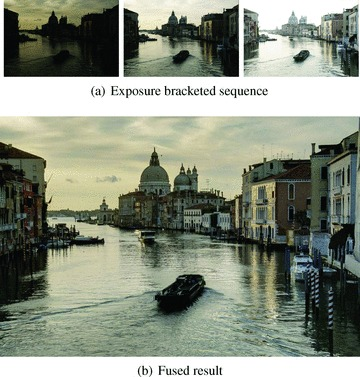
\includegraphics[width=\textwidth]{./Images/Exposure-Fusion.png}
      \caption{Exposure Fusion: \cite{Mertens2008}}
    \end{minipage}
    \hfill
    \begin{minipage}[b]{0.38\linewidth}
      \centering
      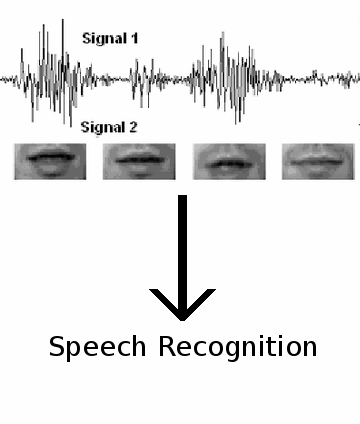
\includegraphics[width=\textwidth]{./Images/SpeechRecognitioncopy.png}
      \caption{Speech Recognition: \cite{Dactu2007}}
    \end{minipage}
    \hfill
  \end{figure}
\end{frame}
% ------------------------------------------------
\begin{frame}
  \frametitle{Example Multimodal Data}
  Remote sensing example: RGB + Elevation map.\\
  From 2015 IEEE Data Fusion Contest.\\
  \cite{DFC2015}\\
  \begin{figure}
    \hfill
    \begin{minipage}[b]{0.40\linewidth}
      \centering
      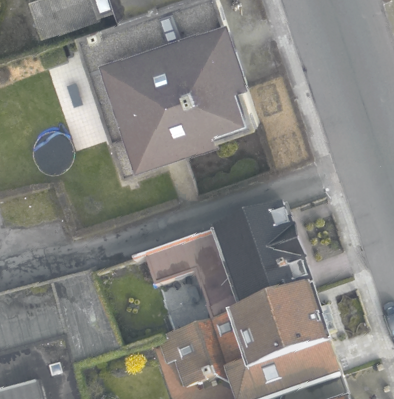
\includegraphics[width=\textwidth]{./Images/DFC2015/optical.png}
      \caption{RGB Data}
    \end{minipage}
    \hfill
    \begin{minipage}[b]{0.40\linewidth}
      \centering
      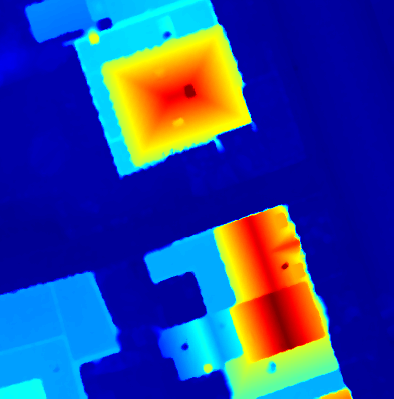
\includegraphics[width=\textwidth]{./Images/DFC2015/lidarColor.png}
      \caption{Lidar Data}
    \end{minipage}
    \hfill
  \end{figure}
\end{frame}

% ------------------------------------------------

\begin{frame}
  \frametitle{Challenges in multimodality}
  Most multimodal methods are developed specifically for one problem, BUT: \\~\\
  %
  \cite{Lahat2015}: ``... a solution that is based on a sufficiently data-driven, model-free approach may turn out to be useful in very different domains.''
  % 
\end{frame}

% ------------------------------------------------


\subsection{Manifold alignment}
\begin{frame}
  \frametitle{Manifold alignment}
  Attempt to address multimodality in general.\\~\\
  % 
  For each modality, view the data as a manifold \\
  (have sets $X^1,X^2,\ldots,X^\ell$. $\ell = $ number of modalities).
  % 
  \begin{figure}
    \hfill
    \begin{minipage}[b]{0.40\linewidth}
      \centering
      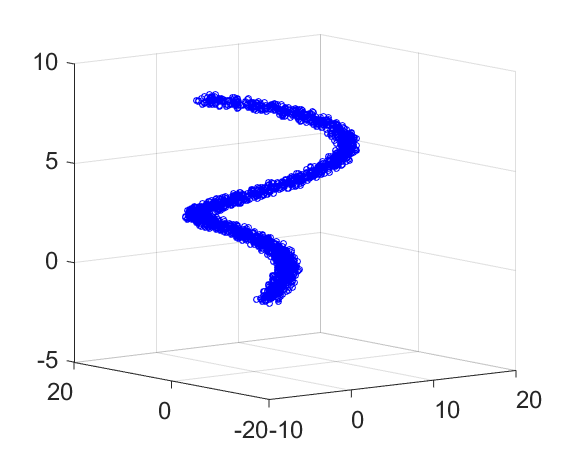
\includegraphics[width=\textwidth]{./Images/KEMA_Example/X1.png}
      \caption{$X^1$}
    \end{minipage}
    \hfill
    \begin{minipage}[b]{0.40\linewidth}
      \centering
      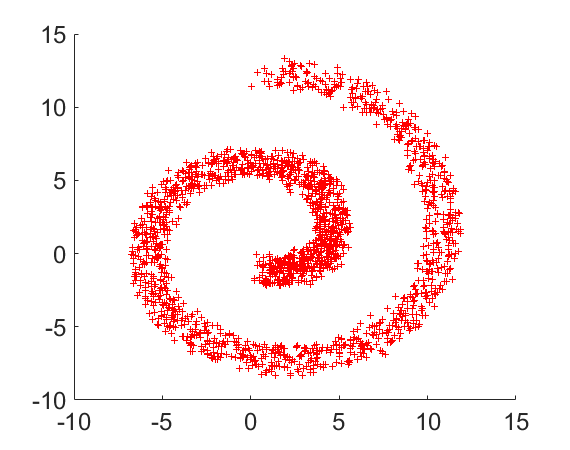
\includegraphics[width=\textwidth]{./Images/KEMA_Example/X2.png}
      \caption{$X^2$}
    \end{minipage}
    \hfill
  \end{figure}
\end{frame}

% ------------------------------------------------
\begin{frame}
  Create a \emph{latent space} $Y$ and maps $X^i\to Y$.
  \begin{figure}
    \hfill
    \begin{minipage}[b]{0.32\linewidth}
      \centering
      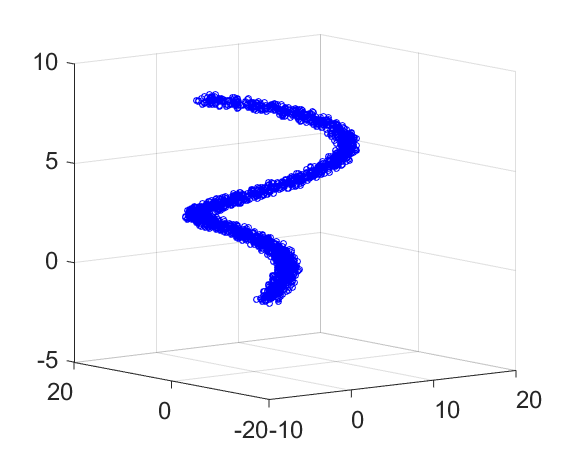
\includegraphics[width=\textwidth]{./Images/KEMA_Example/X1.png}
      \caption{$X^1$}
    \end{minipage}
    \hfill
    \begin{minipage}[b]{0.32\linewidth}
      \centering
      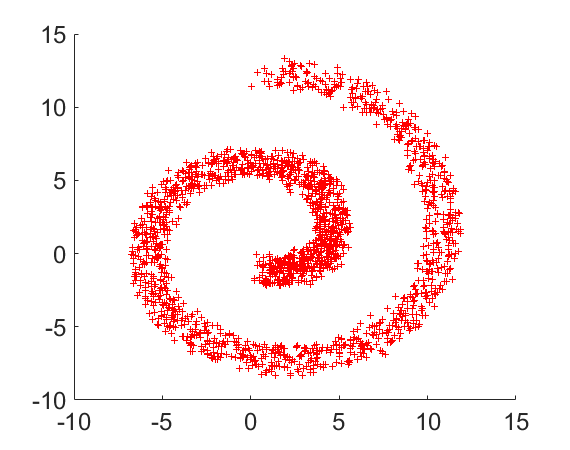
\includegraphics[width=\textwidth]{./Images/KEMA_Example/X2.png}
      \caption{$X^2$}
    \end{minipage}
    \hfill
    \begin{minipage}[b]{0.32\linewidth}
      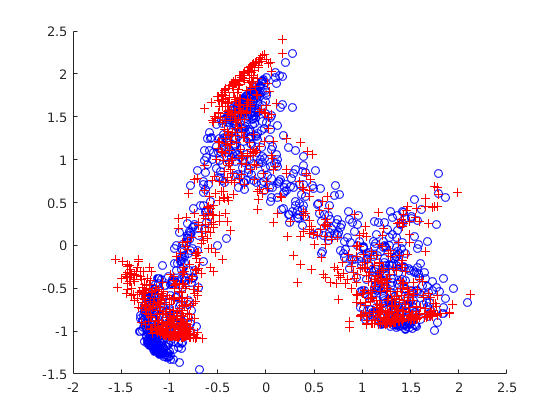
\includegraphics[width=\textwidth]{./Images/KEMA_Example/result.png}
      \caption{Images in latent space}
    \end{minipage}
    \caption{Example from \cite{Tuia2016}}
  \end{figure}
  Compare sets by using the latent space image.
\end{frame}

% ------------------------------------------------

\begin{frame}
  \frametitle{Manifold alignment: Methods from the literature}
  Some examples from the literature:
  \begin{itemize}
  \item \cite{Yeh2014}: Canonical Correlation Analysis, linear or with nonlinear kernel (unsupervised)
  \item \cite{Wang2013}: Graph-based methods (semi-supervised)
  \item \cite{Tuia2016}: Similar to the above with an added nonlinear kernel (semi-supervised)
  \end{itemize}
\end{frame}

% ------------------------------------------------

\begin{frame}
  \frametitle{Manifold alignment: Methods from the literature}
  
  Common theme: Create the latent space by finding and correlating \emph{redundancies} between sets.\\~\\
  % 
  \begin{figure}
    \hfill
    \begin{minipage}[b]{0.32\linewidth}
      \centering
      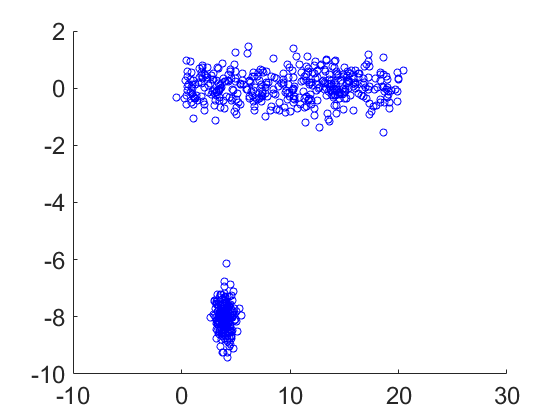
\includegraphics[width=\textwidth]{./Images/Synthetic2/X1.png}
      \caption{$X^1$}
    \end{minipage}
    \hfill
    \begin{minipage}[b]{0.32\linewidth}
      \centering
      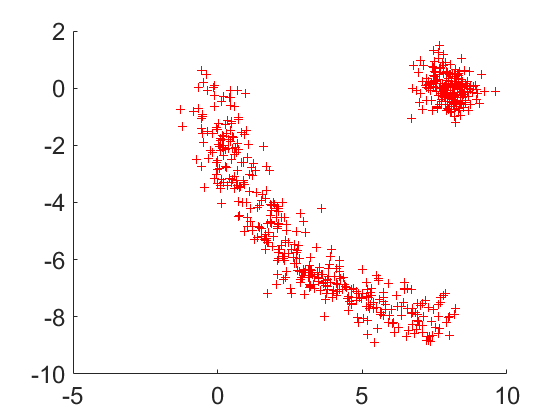
\includegraphics[width=\textwidth]{./Images/Synthetic2/X2.png}
      \caption{$X^2$}
    \end{minipage}
    \hfill
    \begin{minipage}[b]{0.32\linewidth}
      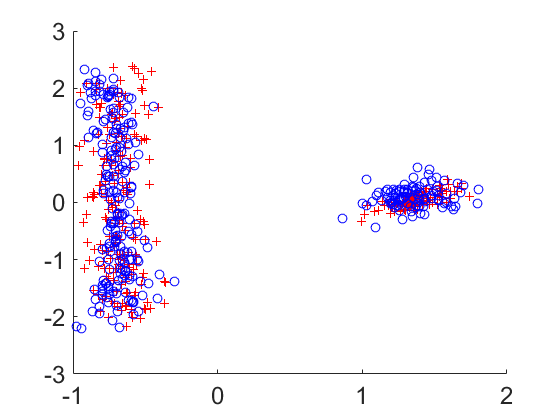
\includegraphics[width=\textwidth]{./Images/Synthetic2/result.png}
      \caption{Images in latent space}
    \end{minipage}
    \caption{Using code from \cite{Tuia2016}}
  \end{figure}

\end{frame}

% ------------------------------------------------

\begin{frame}
  \frametitle{Manifold alignment: Our goal}
  
  Our idea: Can improve on these methods. Find and exploit the unique information that each modality brings.\\~\\
  \begin{figure}
    \hfill
    \begin{minipage}[b]{0.40\linewidth}
      \centering
      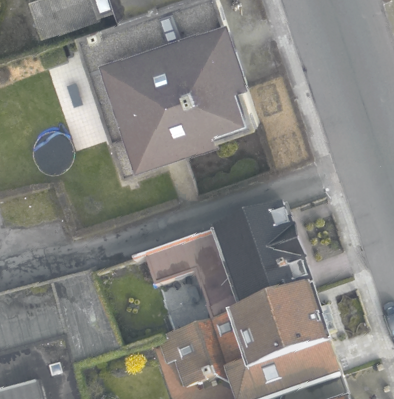
\includegraphics[width=\textwidth]{./Images/DFC2015/optical.png}
      \caption{Distinguish road from grass}
    \end{minipage}
    \hfill
    \begin{minipage}[b]{0.40\linewidth}
      \centering
      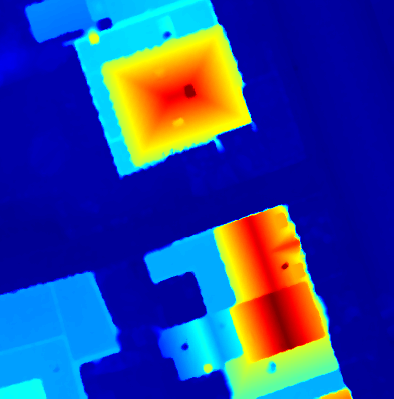
\includegraphics[width=\textwidth]{./Images/DFC2015/lidarColor.png}
      \caption{Distinguish roof from ground}
    \end{minipage}
    \hfill
  \end{figure}
\end{frame}

% ------------------------------------------------

\subsection{Synthetic example}
\begin{frame}
  \frametitle{Synthetic example: Data}
  Ground truth = 3 point clouds in $\mathbb{R}^3$ (100 points per cloud).\\
  Modality 1 = projection onto $xy$-plane.\\
  Modality 2 = projection onto $xz$-plane.\\
  Co-registration assumption: index is input to algorithm.
  \begin{figure}[ht]
    \begin{minipage}[b]{0.30\linewidth}
      \centering
      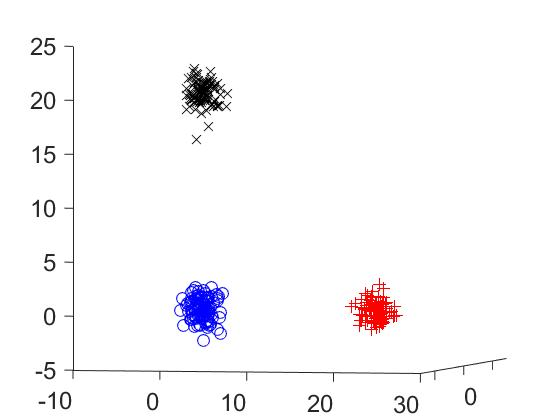
\includegraphics[width=\textwidth]{./Images/Synthetic/groundTruth.jpg}
      \caption{Underlying Data}
    \end{minipage}
    \begin{minipage}[b]{0.30\linewidth}
      \centering
      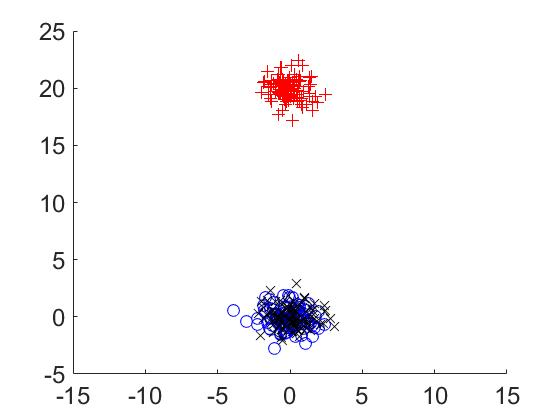
\includegraphics[width=\textwidth]{./Images/Synthetic/set1.jpg}
      \caption{Modality 1}
    \end{minipage}
    \begin{minipage}[b]{0.30\linewidth}
      \centering
      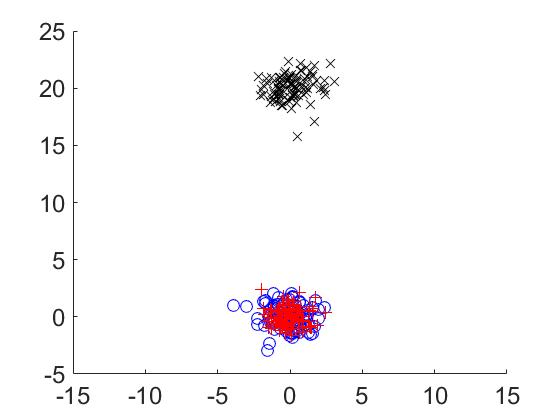
\includegraphics[width=\textwidth]{./Images/Synthetic/set2.jpg}
      \caption{Modality 2}
    \end{minipage}
    \label{fig:SynthData}
  \end{figure}
\end{frame}

% ------------------------------------------------

\begin{frame}
  \frametitle{Synthetic Example: Result of CCA}
  Result of CCA algorithm from \cite{Yeh2014}:
  \begin{figure}[ht]
      \centering
      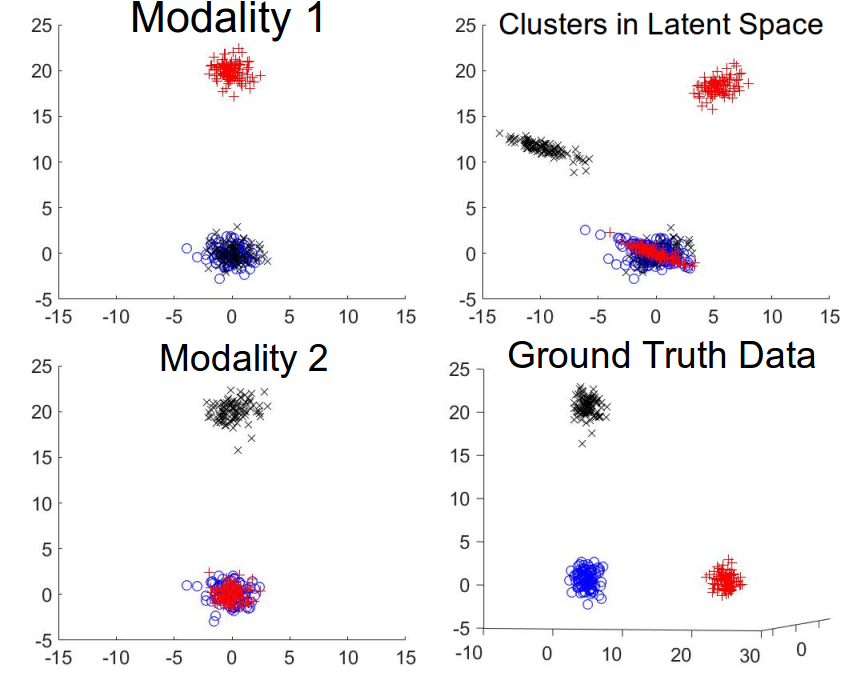
\includegraphics[width=0.8\textwidth]{./Images/Synthetic/fullImage.png}
    \label{fig:SynthData}
  \end{figure}
  % \begin{figure}[ht]
  %   \begin{minipage}[b]{0.3\linewidth}
  %     \centering
  %     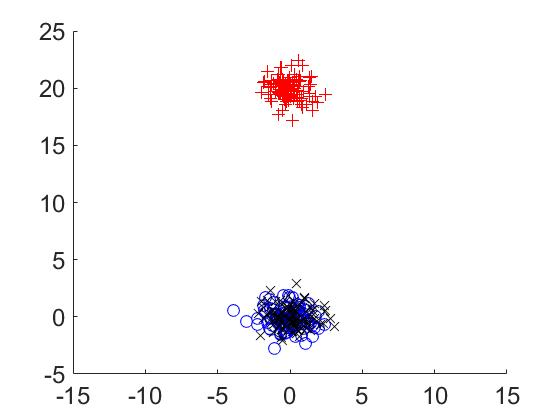
\includegraphics[width=\textwidth]{./Images/Synthetic/set1.jpg}
  %     \caption{Modality 1}
  %   \end{minipage}
  %   \begin{minipage}[b]{0.3\linewidth}
  %     \centering
  %     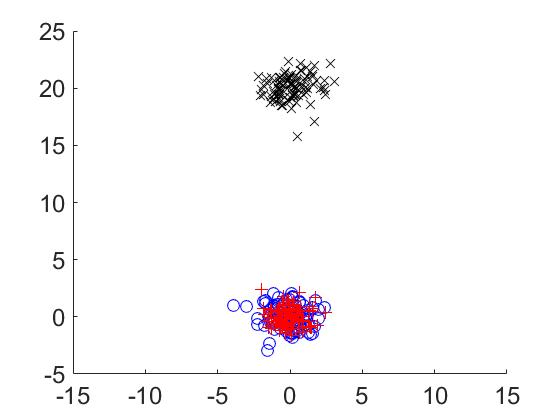
\includegraphics[width=\textwidth]{./Images/Synthetic/set2.jpg}
  %     \caption{Modality 2}
  %   \end{minipage}
  %   \begin{minipage}[b]{0.3\linewidth}
  %     \centering
  %     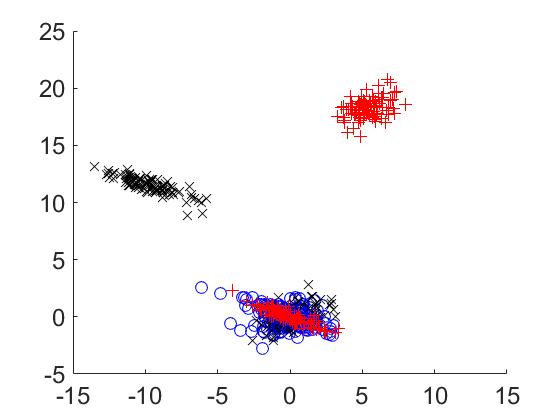
\includegraphics[width=\textwidth]{./Images/Synthetic/clustersLatent.jpg}
  %     \caption{Image in latent space}
  %   \end{minipage}
  %   \label{fig:SynthData}
  % \end{figure}
\end{frame}

% ------------------------------------------------

\section{Multimodal Image Segmentation}
\subsection{Problem setup}
\begin{frame}
  \frametitle{Problem setup}
  We use co-registration assumption and graph Laplacian theory for segmentation of multimodal datasets. \cite{Iyer2017}
  \begin{figure}
    \hfill
    \begin{minipage}[b]{0.40\linewidth}
      \centering
      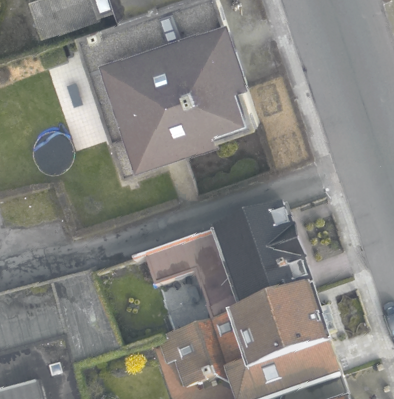
\includegraphics[width=\textwidth]{./Images/DFC2015/optical.png}
      \caption{RGB Data}
    \end{minipage}
    \hfill
    \begin{minipage}[b]{0.40\linewidth}
      \centering
      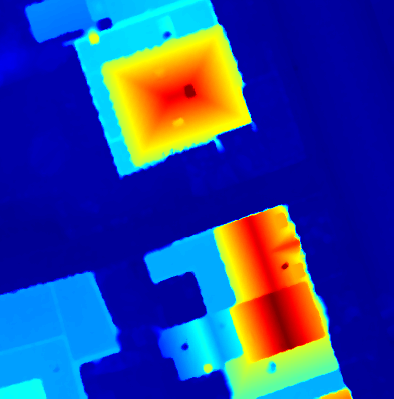
\includegraphics[width=\textwidth]{./Images/DFC2015/lidarColor.png}
      \caption{Lidar Data}
    \end{minipage}
    \hfill
  \end{figure}
\end{frame}

% ------------------------------------------------

\begin{frame}
  \frametitle{Notation}
  From each modality, have a data set $X^k$. $\ell = $ number of modalities.\\~\\
  %
  $N = $ number of observations.\\~\\
  %
  $d_j = $ dimension of set $X^k$. (Can view $X^k \in \mathbb{R}^{N\times d_k}$). \\~\\
  %
  From co-registration assumption: \\
  $i$-th point in $X^{k_1}$ corresponds to $i$-th point in $X^{k_2}$. \\
  Create concatenated set $X = (X^1,X^2,\ldots,X^\ell) \subseteq \mathbb{R}^{N\times\left(d_1+\cdots+d_\ell\right)}$. \\~\\
  %
  $x_i = $ element $i$ from $X$. $x_i^k = $ element $i$ from $X^k$.
\end{frame}

% ------------------------------------------------

\subsection{Multimodal weights}
\begin{frame}
  \frametitle{Graph Representation: Background}
  When using a single modality: \\~\\
  \hspace*{20pt} For each pair $x_i,x_j\in X$, define a \emph{weight} $w_{ij}$ that measures \hspace*{20pt} the similarity between the points. \\~\\
  \hspace*{20pt} $\implies$ represent data as $N \times N$ weight matrix $W$. \\~\\
  \hspace*{20pt} Common similarity measure from the literature: RBF kernel
    \[w_{ij} = \text{exp}\left(-\norm{x_i - x_j}^2 / \sigma \right).\]
  Need to adapt this to multimodal data.
\end{frame}

% ------------------------------------------------

\begin{frame}
  \frametitle{Multimodal Weight Matrix}
  For each modality $X^k$, calculate the distance matrix $E^k$ via
  \[E^k_{ij} = \norm{x^k_i - x^k_j}.\]
  $\norm{\cdot}$ chosen based on the details of the modality.\\~\\
  %
  (in our examples $\norm{\cdot}$ is the 2-norm) \\~\\
  %
  Scale each matrix by standard deviation (nondimensionalization)
  \[\bar{E}^k = \frac{E^k}{\text{std}\left(E^k\right)}.\]
\end{frame}

% ------------------------------------------------

\begin{frame}
  \frametitle{Multimodal Weight Matrix}
  Define \[w_{ij} = \text{exp}\left(-\max\left(\bar{E}^1_{ij},\ldots,\bar{E}^k_{ij}\right)/\sigma\right).\]
  Heuristics:
  \begin{itemize}
  \item Standard deviation scaling allows us to directly compare $\bar{E}^{k_1},\bar{E}^{k_2}$ with reasonable results.
  \item Because of the $\max$, elements are similar under this measure only if they are similar in each modality.
  \end{itemize}
\end{frame}
% ------------------------------------------------
\subsection{Feature extraction with graph Laplacian}
\begin{frame}
  \frametitle{Graph min-cut}
  Use weights $W$ to segment $X$ into $A_1,\ldots,A_k$. We want to
  \begin{itemize}\item group nodes with high similarity (weight) together
  \item ensure each set is a reasonable size
  \end{itemize}
  Use the \emph{Normalized graph-cut}  
  \[\text{Ncut}(A_1,\ldots,A_k) = \frac{1}{2}\sum_{j=1}^k \frac{W(A_j,A_j^c)}{vol(A_j)}.\]
  \[W(A,B) = \sum_{i \in A, j \in B} w_{ij}.\]
  \[vol(A) = \sum_{i \in A, j \in X} w_{ij}.\]
  Exact min-cut solution is computationally infeasible.
\end{frame}

% ------------------------------------------------
\begin{frame}
  \frametitle{Graph Laplacian}
  A well-known approximation for graph min-cut: \\
  eigenvectors of the graph Laplacian $L$.\\
  \[L = I -D^{-1/2}WD^{-1/2},\]
  where $D = N\times N$ diagonal matrix (degree matrix), with
  \[d_{ii} = \sum_{j=1}^n w_{ij}.\]
\end{frame}
% ------------------------------------------------

\begin{frame}
  \frametitle{Feature extraction}
  Result of \cite{vonLuxburg07}
  \begin{align*}
    \text{eigenvectors of }L &\iff \text{ features extracted from data}
  \end{align*}
  Can use eigenvectors for a variety of applications. \\~\\
  %
  Our results: K-means on eigenvectors $\to$ segmentation \\
  (this is called Spectral Clustering). \\~\\
  %
  Future work: Apply graph MBO \cite{Merkurjev13} instead.
\end{frame}
% ------------------------------------------------

\subsection{Nystr\"{o}m Extension}
\begin{frame}
  \frametitle{Nystr\"{o}m Extension}
  As $\abs{X}$ becomes large, computing the $\abs{X}\times \abs{X}$ weight matrix $W$ becomes prohibitive. \\~\\
  Instead choose $A \subseteq X$ \emph{landmark nodes} with $\abs{A}\ll\abs{X}$. Up to permutation, we have
  \[  W = \begin{pmatrix} W_{A,A} & W_{A,A^c} \\ W_{A^c,A} & W_{A^c,A^c}
    \end{pmatrix}.\]
  \cite{Fowlkes04}: \\
  Approximate graph Laplacian eigenvectors using only $W_{A,A},W_{A^c,A}$.
  \[  W \approx \begin{pmatrix} W_{A,A} \\ W_{A^c,A} \end{pmatrix}
    W_{AA}^{-1} \begin{pmatrix} W_{A,A} & W_{A,A^c}\end{pmatrix}.\]
  Compute and store matrices of size at most $\abs{X}\times\abs{A}$.
\end{frame}

% ------------------------------------------------
\section{Results}
\subsection{Synthetic example revisited}
\begin{frame}
  \frametitle{Synthetic example: Data}
  Synthetic example:\\
  Ground truth = 3 point clouds in $\mathbb{R}^3$ (100 points per cloud).\\
  Modality 1 = projection onto $xy$-plane.\\
  Modality 2 = projection onto $xz$-plane.
  \begin{figure}[ht]
    \begin{minipage}[b]{0.3\linewidth}
      \centering
      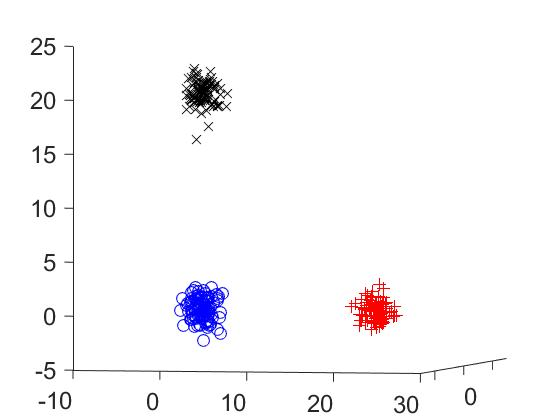
\includegraphics[width=\textwidth]{./Images/Synthetic/groundTruth.jpg}
      \caption{Ground Truth}
    \end{minipage}
    \begin{minipage}[b]{0.3\linewidth}
      \centering
      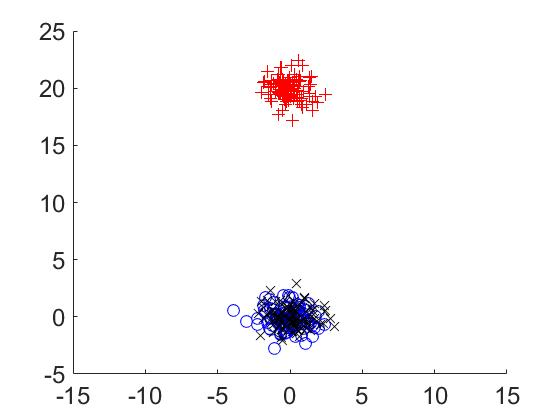
\includegraphics[width=\textwidth]{./Images/Synthetic/set1.jpg}
      \caption{Modality 1}
    \end{minipage}
    \begin{minipage}[b]{0.3\linewidth}
      \centering
      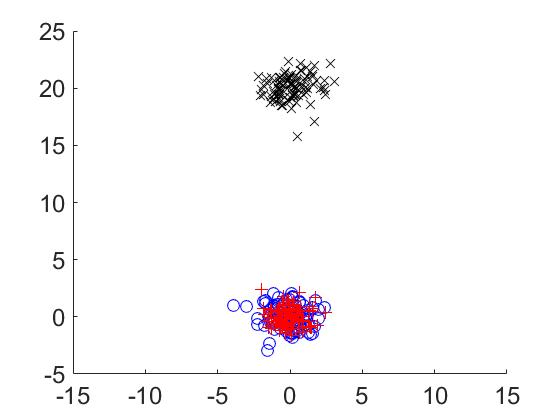
\includegraphics[width=\textwidth]{./Images/Synthetic/set2.jpg}
      \caption{Modality 2}
    \end{minipage}
    \label{fig:SynthData}
  \end{figure}
\end{frame}

% ------------------------------------------------

\begin{frame}
  \frametitle{Synthetic Example: Result of Our Method}
  Result of our multimodal graph-based algorithm on earlier example: \\
  Plotting first 2 eigenvectors.
  \begin{figure}
    \centering
    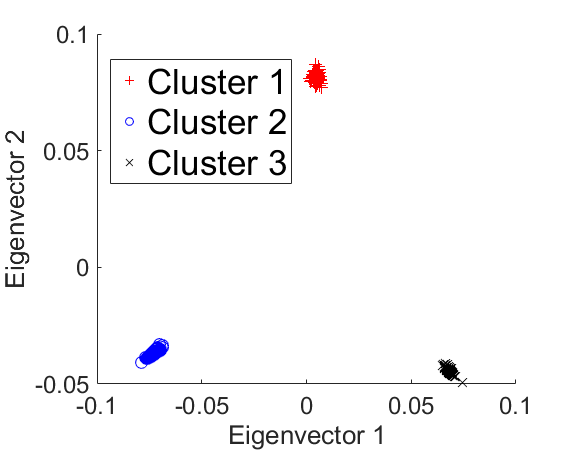
\includegraphics[width=0.5\linewidth]{./Images/Synthetic/clustersGraph.png}
    \caption{2 eigenvectors of graph Laplacian}
  \end{figure}
\end{frame}
% ------------------------------------------------

\subsection{DFC2015 data}
\begin{frame}
  \frametitle{Data}
  Our algorithm applied to \cite{DFC2015} dataset.
  \begin{figure}[ht]
    \begin{minipage}[b]{0.45\linewidth}
      \centering
      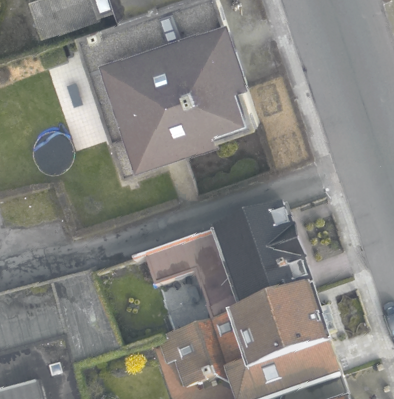
\includegraphics[width=\textwidth]{./Images/DFC2015/optical.png}
      \caption{RGB Modality}
    \end{minipage}
    \begin{minipage}[b]{0.45\linewidth}
      \centering
      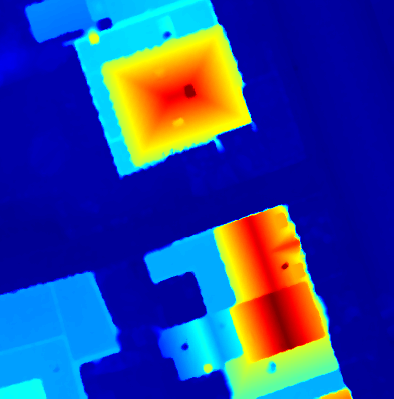
\includegraphics[width=\textwidth]{./Images/DFC2015/lidarColor.png}
      \caption{Lidar Modality}
    \end{minipage}
  \end{figure}
\end{frame}

% ------------------------------------------------

\begin{frame}
  \frametitle{Results}
  \begin{figure}[ht]
    \begin{minipage}[b]{0.3\linewidth}
      \centering
      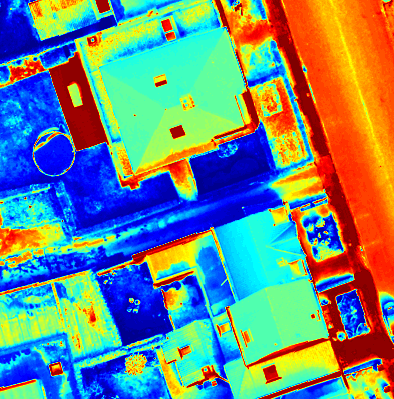
\includegraphics[width=\textwidth]{./Images/DFC2015/evec1.png}
    \end{minipage}
    \begin{minipage}[b]{0.3\linewidth}
      \centering
      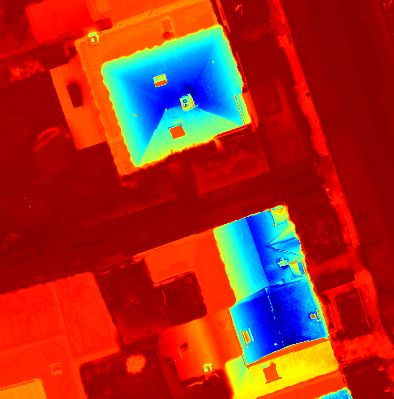
\includegraphics[width=\textwidth]{./Images/DFC2015/evec2.png}
    \end{minipage}
    \begin{minipage}[b]{0.3\linewidth}
      \centering
      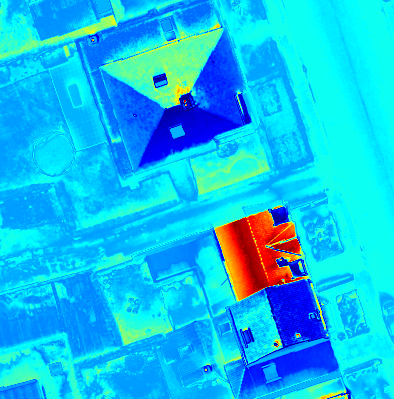
\includegraphics[width=\textwidth]{./Images/DFC2015/evec4.png}
    \end{minipage}
    \caption{Example eigenvectors of graph Laplacian}
  \end{figure}
\end{frame}

% ------------------------------------------------

\begin{frame}
  \frametitle{Results}
  Spectral Clustering result (unsupervised). $m = 6$ classes.
  \begin{figure}[ht]
    \begin{minipage}[b]{0.45\linewidth}
      \centering
      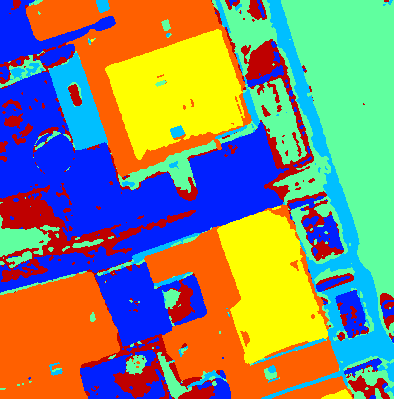
\includegraphics[width=\textwidth]{./Images/DFC2015/K.png}
      \caption{Classes}
    \end{minipage}
    \begin{minipage}[b]{0.45\linewidth}
      \centering
      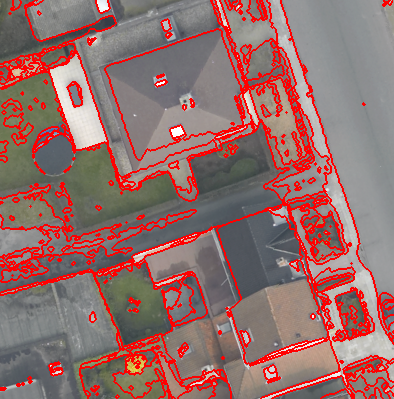
\includegraphics[width=\textwidth]{./Images/DFC2015/segmentation.png}
      \caption{Regions on original image}
    \end{minipage}
  \end{figure}
\end{frame}

% ------------------------------------------------

\subsection{Umbrella data}
\begin{frame}
  \frametitle{Data}
  Our algorithm applied to \cite{Scharstein2014} dataset.
  \begin{figure}[ht]
    \begin{minipage}[b]{0.45\linewidth}
      \centering
      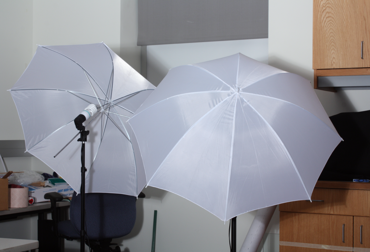
\includegraphics[width=\textwidth]{./Images/Umbrella/optical.png}
      \caption{RGB Modality}
    \end{minipage}
    \begin{minipage}[b]{0.45\linewidth}
      \centering
      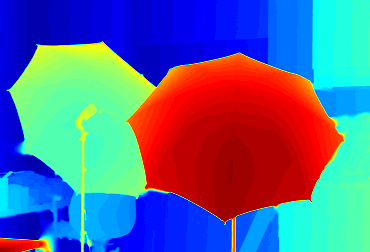
\includegraphics[width=\textwidth]{./Images/Umbrella/lidarColor.png}
      \caption{Lidar Modality}
    \end{minipage}
  \end{figure}
\end{frame}

% ------------------------------------------------

\begin{frame}
  \frametitle{Results}
  \begin{figure}[ht]
    \begin{minipage}[b]{0.40\linewidth}
      \centering
      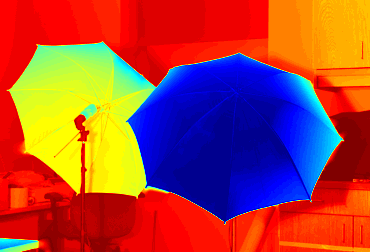
\includegraphics[width=\textwidth]{./Images/Umbrella/evecColor.png}
    \end{minipage}
    \begin{minipage}[b]{0.40\linewidth}
      \centering
      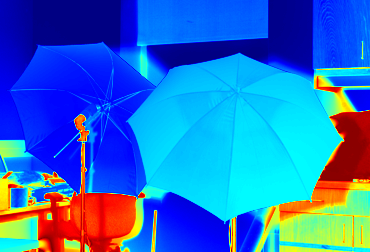
\includegraphics[width=\textwidth]{./Images/Umbrella/evec2.png}
    \end{minipage}
    \vfill
    \begin{minipage}[b]{0.40\linewidth}
      \centering
      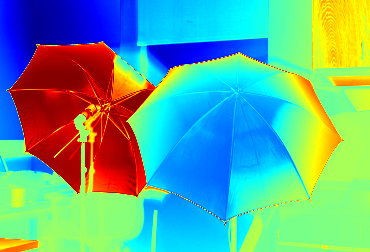
\includegraphics[width=\textwidth]{./Images/Umbrella/evec3.png}
    \end{minipage}
    \caption{Example eigenvectors of graph Laplacian}
  \end{figure}
\end{frame}

% ------------------------------------------------

\begin{frame}
  \frametitle{Results}
  Spectral Clustering result (unsupervised). $m = 8$ classes.
  \begin{figure}[ht]
    \begin{minipage}[b]{0.45\linewidth}
      \centering
      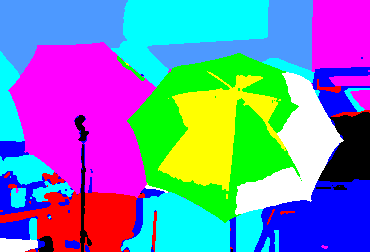
\includegraphics[width=\textwidth]{./Images/Umbrella/clustering.png}
      \caption{Classes}
    \end{minipage}
    \begin{minipage}[b]{0.45\linewidth}
      \centering
      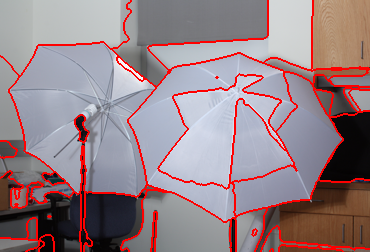
\includegraphics[width=\textwidth]{./Images/Umbrella/segmentation.png}
      \caption{Regions on original image}
    \end{minipage}
  \end{figure}
\end{frame}
% ------------------------------------------------
\section{Future Work: Graph Matching}
\begin{frame}
  \frametitle{Graph Matching}
  Goal: Remove or weaken the coregistration assumption.\\~\\
  %
  Current idea: Graph matching. \\~\\
  % 
  View each dataset as a (weighted) graph.\\
  Try to match nodes with similar structure.
\end{frame}
% ------------------------------------------------

% \begin{frame}
%   \frametitle{Graph Matching Example}
%   \begin{figure}[ht]
%     \centering
%     \begin{minipage}[b]{0.40\linewidth}
%       \centering
%       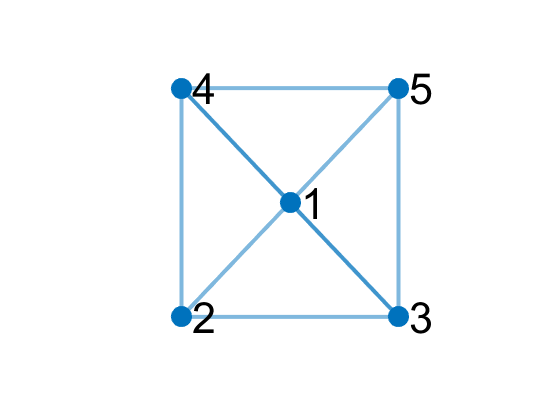
\includegraphics[width=\textwidth]{./Images/GraphMatch/structureEx1.png}
%       \caption{Graph 1}
%     \end{minipage}
%     \begin{minipage}[b]{0.40\linewidth}
%       \centering
%       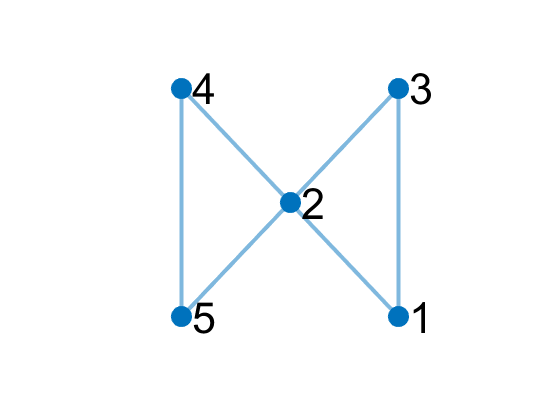
\includegraphics[width=\textwidth]{./Images/GraphMatch/structureEx2.png}
%       \caption{Graph 2}
%     \end{minipage}
%   \end{figure}
%   Any reasonable matching sends $1 \to 2$. \\~\\
%   %
%   Other nodes can be matched in any way (symmetry).
% \end{frame}

% ------------------------------------------------
\subsection{Graph matching}
\begin{frame}
  \frametitle{Problem Setup}
  Two weighted graphs, $G_1,G_2$, with weight matrices $W_1,W_2$.\\~\\
  %
  For now, $\abs{G_1} = \abs{G_2} = N$.\\~\\
  %
  Search for a graph isomorphism $G_1\to G_2$ preserving edge weights.
  \begin{figure}[ht]
    \centering
    \begin{minipage}[b]{0.40\linewidth}
      \centering
      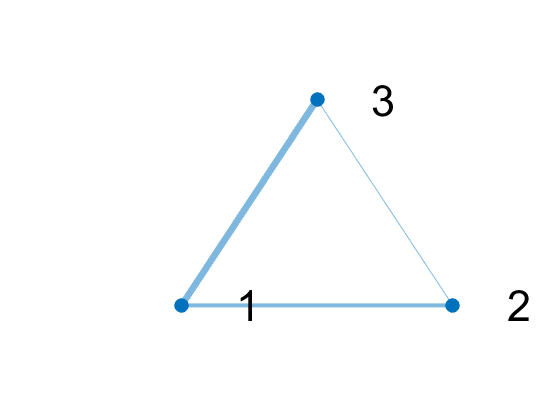
\includegraphics[width=\textwidth]{./Images/GraphMatch/isom1.png}
    \end{minipage}
    \begin{minipage}[b]{0.40\linewidth}
      \centering
      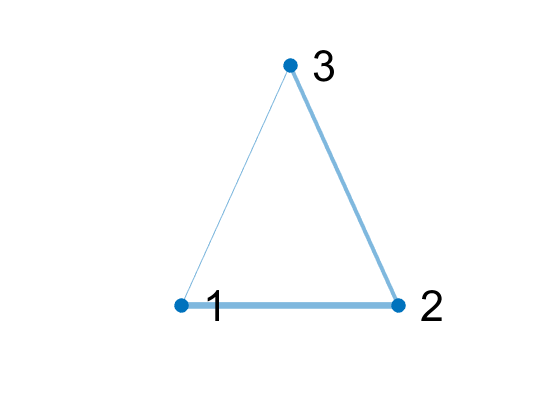
\includegraphics[width=\textwidth]{./Images/GraphMatch/isom2.png}
    \end{minipage}
  \end{figure}
  Best isomorphism is $1 \to 2$, $2 \to 3$, $3 \to 1$.
\end{frame}

% ------------------------------------------------

\begin{frame}
  \frametitle{Problem Setup}
  Isomorphism $G_1\to G_2$ corresponds to a permutation on nodes. Have $P$ the corresponding permutation matrix. Want to minimize
  \[\norm{W_1 - PW_2P^T}^2_F.\]
  Exact solution is too expensive. Can solve using graph Laplacian trick from \cite{Umeyama1988,Knossow2009}.\\~\\
\end{frame}

% ------------------------------------------------

\begin{frame}
  \frametitle{Relaxation}
  Relax problem to
  \[Q^* = \text{argmin}_{QQ^T=I}\norm{W_1 - QW_2Q^T}^2_F.\]
  Let $L_1,L_2$ the graph Laplacians corresponding to $W_1,W_2$ \\~\\
  $U_1,U_2$ the corresponding matrices of eigenvectors. \\~\\
  Then $Q^* = U_1SU_2^T$.\\~\\
  $S$ is a diagonal matrix with entries of $\pm 1$ to account for sign ambiguity in eigenvectors.
\end{frame}

% ------------------------------------------------

\begin{frame}
  \frametitle{Heuristics}
  Recall from graph Laplacian
  \begin{align*}
    \text{column of }U_i &\iff \text{ feature extracted from data} \\
    \text{row of }U_i &\iff \text{ image of data point in new feature space}.
  \end{align*}
  Match rows of $U_1$ to rows of $U_2$ by considering $U_1U_2^T$. \\~\\
\end{frame}

% ------------------------------------------------

\begin{frame}
  \frametitle{Matching Algorithm}
  $Q^*_{ij}$ gives the similarity between node $i$ of $G_1$ and node $j$ of $G_2$. \\~\\
  Choose a permutation $p: \{1,2,\ldots,N\} \to \{1,2,\ldots,N\}$ via
  \[\text{argmax}_{\text{permutations }p}\sum_{i=1}^N Q^*_{i,p(i)}.\]
  Hungarian algorithm finds this in $O(N^3)$ \cite{Munkres1957}.
\end{frame}

% ------------------------------------------------

% \begin{frame}
%   \frametitle{Example Calculation}
%   Say we have $N=6$ and calculated:
%   \[Q^* = \begin{pmatrix}
%    -0.1629 &  -0.1711 &  -0.1703 &   0.3426 &   0.3717 &  -0.2100\\
%    -0.1647 &  -0.1662 &  -0.1677 &   0.2966 &   0.3192 &  -0.1172\\
%    -0.1660 &  -0.1653 &  -0.1657 &  -0.1477 &  -0.1861 &   0.8308\\
%    -0.4579 &   0.6860 &   0.2665 &  -0.1787 &  -0.1480 &  -0.1678\\
%     0.4939 &  -0.1039 &   0.1196 &  -0.6689 &   0.3080 &  -0.1486\\
%     0.4577 &  -0.0795 &   0.1176 &   0.3561 &  -0.6647 &  -0.1872\\
%   \end{pmatrix}\]
%   Then \[P^* = \begin{pmatrix}
%       0&0&0&1&0&0\\
%       0&0&0&0&1&0\\
%       0&0&0&0&0&1\\
%       0&1&0&0&0&0\\
%       1&0&0&0&0&0\\
%       0&0&1&0&0&0\\
%     \end{pmatrix}
%   \]
% \end{frame}

% ------------------------------------------------

\begin{frame}
  \frametitle{Benefits of Graph Matching}
  Benefits of Graph Matching
  \begin{enumerate}
  \item Invariant under conformal maps.
    \begin{itemize}
    \item scaling, shifts, rotations, etc.
    \item robust to continuous deformation.
    \end{itemize}
  \item A precise number representing similarity between nodes gives us many options.
    \begin{itemize}
    \item Thresholding
    \item Hierarchical matching
    \end{itemize}
  \item Easy extension to the case $\abs{G_1}\neq\abs{G_2}$.
  \end{enumerate}
\end{frame}

% ------------------------------------------------

\begin{frame}
  \frametitle{Example Matching}
  \begin{figure}
    \centering
    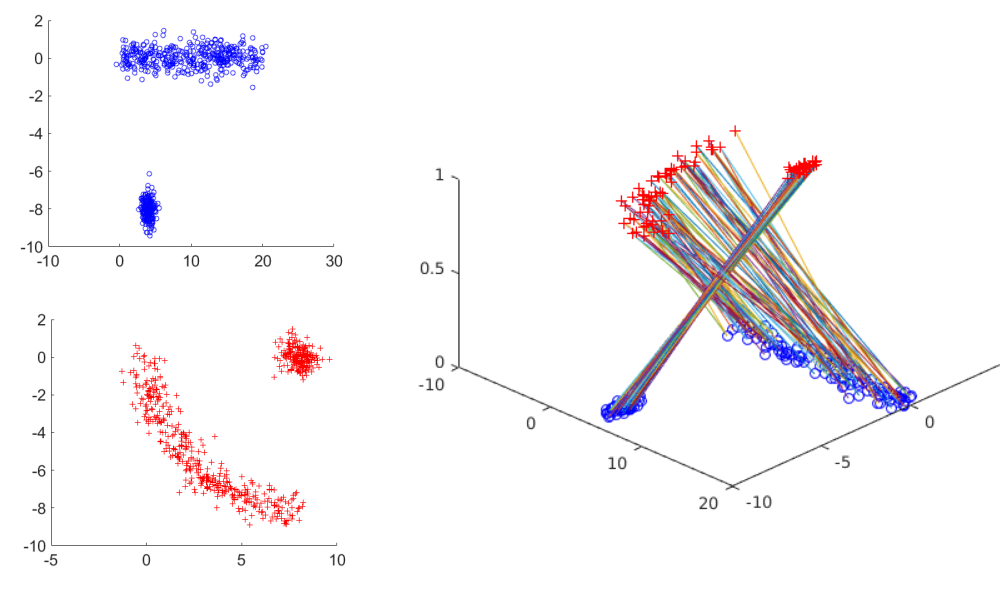
\includegraphics[width = 0.9\textwidth]{./Images/GraphMatch/CombinePic/combinepic.png}
    \caption{Graph Match on Synthetic Data}
  \end{figure}
\end{frame}

% ------------------------------------------------

\begin{frame}
  \frametitle{Change Detection}
  One possible application: Change detection. \\~\\
  % 
  Given images $X$ and $Y$ of the same scene, compare coregistration against results of graph matching. Use this to pick out large changes between $X, Y$.\\~\\
  %
  From graph matching, get a permutation
  \[\rho: \{1,\ldots,n\} \to \{1,\ldots,n\}.\]
  %
  Compare $x_i$ to $x_{\rho(i)}$, and $y_i$ to $y_{\rho(i)}$. \\~\\
\end{frame}

% ------------------------------------------------

% \begin{frame}
%   \frametitle{Change Detection}
%   Let $X = \{x_1, x_2, \ldots, x_n\}$, $Y = \{y_1,y_2,\ldots,y_n\}$. \\~\\
%   A poor match $\implies$ some change occured. \\~\\
% \end{frame}

% % ------------------------------------------------

\begin{frame}
  \frametitle{Change Detection Example}
  \begin{figure}
    \begin{minipage}[b]{0.40\linewidth}
      \centering
      
\includegraphics[width=\textwidth]{./Images/GraphMatch/dataAfter.png}
      \caption{Image $X$}
    \end{minipage}
    \hfill
    \begin{minipage}[b]{0.40\linewidth}
      \centering
      
\includegraphics[width=\textwidth]{./Images/GraphMatch/dataBefore.png}
      \caption{Image $Y$}
    \end{minipage}
    \vfill
    \begin{minipage}[b]{0.40\linewidth}
      \centering
      
\includegraphics[width=\textwidth]{./Images/GraphMatch/naivediff.png}
      \caption{Naive difference $\norm{X-Y}$}
    \end{minipage}
    \hfill
    \begin{minipage}[b]{0.40\linewidth}
      \centering
      
\includegraphics[width=\textwidth]{./Images/GraphMatch/normMap.png}
      \caption{$\norm{x_i - x_{\rho(i)}}$}
    \end{minipage}
  \end{figure}
\end{frame}

% ------------------------------------------------

\begin{frame}
  \frametitle{Future directions}
  Possible directions for future work
  \begin{enumerate}
  \item Improve image segmentation using graph MBO.
  \item Change detection using graph matching.
  \item Push performance of graph matching.
  \end{enumerate}
\end{frame}

% ------------------------------------------------

\section{References}
\begin{frame}[allowframebreaks]
  \frametitle{References}
  \footnotesize{
    \begin{thebibliography}{99} % Beamer does not support BibTeX so references must be inserted manually as below
    \bibitem[Mertens et al, CGF, 2008]{Mertens2008} Tom Mertens and J. Kautz and Frank Van Reeth
      \newblock Exposure Fusion: A Simple and Practical Alternative to High Dynamic Range Photography
      \newblock \emph{Computer Graphics Forum} 28(1):161 - 171
      % 
      % 
    \bibitem[Datcu et al, IEEE CVPR 2007]{Dactu2007} D. Datcu and Z. Yang and L. Rothkrantz (2007)
      \newblock Multimodal workbench for automatic surveillance applications
      \newblock \emph{2007 IEEE Conference on Computer Vision and Pattern Recognition} 1-2
      % 
      % 
    \bibitem[Lahat et al, IEEE 2015]{Lahat2015} Lahat, Dana and Adal{\i}, T{\"u}lay and Jutten, Christian (2015)
      \newblock Multimodal Data Fusion: An Overview of Methods, Challenges and Prospects
      \newblock \emph{Proceedings of the IEEE } 103(9), 1449-1477
      % 
      % 
    \bibitem[Yeh et al, IEEE TIP 2014]{Yeh2014} Yi-Ren Yes and Chun-Hao Huang and Yu-Chiang Frank Wang
      \newblock Heterogeneous Domain Adaptation and Classification by Exploiting the Correlation Subspace
      \newblock \emph{IEEE Transactions on Image Processing} 23(5), 2009-2018
      % 
      % 
    \bibitem[Wang et al, IJCAI 2013]{Wang2013} Wang, Chang and Mahadevan, Sridhar (2013)
      \newblock Manifold Alignment Preserving Global Geometry
      \newblock \emph{Proceedings of the Twenty-Third International Joint Conference on Artificial Intelligence} IJCAI '13, 1743-1749
      % 
      % 
    \bibitem[Tuia et al, PLOS ONE 2016]{Tuia2016} Tuia, Devis AND Camps-Valls, Gustau (2016)
      \newblock Kernal Manifold Alignment for Domain Adaptation
      \newblock \emph{PLOS ONE} 11, 1-25
      %
      %
    \bibitem[Bampos-Taberner et al, IEEE J-STARS 2016]{DFC2015} M. Campos-Taberner and A. Romero-Soriano and C. Gatta and G. Camps-Valls and A. Lagrange and B. Le Saux and A. Beaupère and A. Boulch and A. Chan-Hon-Tong and S. Herbin and H. Randrianarivo and M. Ferecatu and M. Shimoni and G. Moser and D. Tuia (2015)
      \newblock Processing of Extremely High-Resolution LiDAR and RGB Data: Outcome of the 2015 IEEE GRSS Data Fusion Contest \#8211;Part A: 2-D Contest
      \newblock \emph{IEEE Journal of Selected Topics in Applied Earth Observations and Remote Sensing} 9(12), 5547-5559
      %
      %
    \bibitem[Iyer et al., Accepted Paper, ICIP 2017]{Iyer2017} Iyer, Geoffrey and Chanussot, Jocelyn and Bertozzi, Andrea (2017).
      \newblock A Graph-Based Approach for Feature Extraction and Segmentation of Multimodal Images
      \newblock Preprint
      %
      %
    \bibitem[Scharstein et al., GCPR 2014]{Scharstein2014} Daniel Scharstein and Heiko Hirschm\"{u}ller and York Kitajima and Greg Krathwohl and Nera Ne\v{s}i\'{c} and Xi Wang and Porter Westling (2014)
      \newblock High-resolution stereo datasets with subpixel-accurate ground truth
      \newblock \emph{Proceedings of the 36th German Conference on Pattern Recognition} 31-42
      %
      %
    \bibitem[Umeyama, IEEE TPAMI 1988]{Umeyama1988} Umeyama, S. (1988)
      \newblock An Eigendecomposition Approach to Weighted Graph Matching Problems
      \newblock \emph{IEEE Trans. Pattern Anal. Mach. Intell.}, 10(5), 695-703
      %
      %
    \bibitem[Knossow et al., GbRPR 2009]{Knossow2009} Knossow, David and Sharma, Avinash and Mateus, Diana and Horaud, Radu (2009)
      \newblock Inexact Matching of Large and Sparse Graphs Using Laplacian Eigenvectors
      \newblock Graph-Based Representations in Pattern Recognition: 7th IAPR-TC-15 International Workshop, 2009. Proceedings
      %
      %
    \bibitem[vonLuxburg, Stat Comput 2007]{vonLuxburg07} vonLuxburg, Ulrike (2007)
      \newblock A tutorial on spectral clustering
      \newblock Statistics and Computing, 17(4), 395-416
      %
      %
    \bibitem[Merkurjev, SIIMS 2013]{Merkurjev13} Ekaterina Merkurjev and Tijana Kostic and Andrea L Bertozzi (2013)
      \newblock An MBO scheme on graphs for classification and image processing
      \newblock SIAM Journal on Imaging Sciences, 6(4), 1903-1930
      %
      %
    \bibitem[Fowlkes et al., IEEE TPAMI 2004]{Fowlkes04} Charless Fowlkes and Serge Belongie and Fan Chung and Jitendra Malik (2004)
      \newblock Spectral Grouping Using the Nystrom Method
      \newblock IEEE Transactions on Pattern Analysis and Machine Intelligence, 26(2)
      %
      %
    \bibitem[Munkres, SIAM 1957]{Munkres1957} J. Munkres (1957)
      \newblock Algorithms for the Assignment and Transportation Problems
      \newblock Journal of the Society for Industrial and Applied Mathematics, 5(1):32–38
    \end{thebibliography}
  }
\end{frame}

% ------------------------------------------------

% \section{Templates}
% \subsection{Template Stuff}
% \begin{frame}
%   \frametitle{Bullet Points}
%   \begin{itemize}
%   \item Lorem ipsum dolor sit amet, consectetur adipiscing elit
%   \item Aliquam blandit faucibus nisi, sit amet dapibus enim tempus eu
%   \item Nulla commodo, erat quis gravida posuere, elit lacus lobortis est, quis porttitor odio mauris at libero
%   \item Nam cursus est eget velit posuere pellentesque
%   \item Vestibulum faucibus velit a augue condimentum quis convallis nulla gravida
%   \end{itemize}
% \end{frame}

% % ------------------------------------------------

% \begin{frame}
%   \frametitle{Blocks of Highlighted Text}
%   \begin{block}{Block 1}
%     Lorem ipsum dolor sit amet, consectetur adipiscing elit. Integer lectus nisl, ultricies in feugiat rutrum, porttitor sit amet augue. Aliquam ut tortor mauris. Sed volutpat ante purus, quis accumsan dolor.
%   \end{block}

%   \begin{block}{Block 2}
%     Pellentesque sed tellus purus. Class aptent taciti sociosqu ad litora torquent per conubia nostra, per inceptos himenaeos. Vestibulum quis magna at risus dictum tempor eu vitae velit.
%   \end{block}

%   \begin{block}{Block 3}
%     Suspendisse tincidunt sagittis gravida. Curabitur condimentum, enim sed venenatis rutrum, ipsum neque consectetur orci, sed blandit justo nisi ac lacus.
%   \end{block}
% \end{frame}

% % ------------------------------------------------

% \begin{frame}
%   \frametitle{Multiple Columns}
%   \begin{columns}[c] % The "c" option specifies centered vertical alignment while the "t" option is used for top vertical alignment

%     \column{.45\textwidth} % Left column and width
%     \textbf{Heading}
%     \begin{enumerate}
%     \item Statement
%     \item Explanation
%     \item Example
%     \end{enumerate}

%     \column{.5\textwidth} % Right column and width
%     Lorem ipsum dolor sit amet, consectetur adipiscing elit. Integer lectus nisl, ultricies in feugiat rutrum, porttitor sit amet augue. Aliquam ut tortor mauris. Sed volutpat ante purus, quis accumsan dolor.

%   \end{columns}
% \end{frame}

% % ------------------------------------------------

% \begin{frame}
%   \frametitle{Table}
%   \begin{table}
%     \begin{tabular}{l l l}
%       \toprule
%       \textbf{Treatments} & \textbf{Response 1} & \textbf{Response 2}\\
%       \midrule
%       Treatment 1 & 0.0003262 & 0.562 \\
%       Treatment 2 & 0.0015681 & 0.910 \\
%       Treatment 3 & 0.0009271 & 0.296 \\
%       \bottomrule
%     \end{tabular}
%     \caption{Table caption}
%   \end{table}
% \end{frame}

% % ------------------------------------------------

% \begin{frame}
%   \frametitle{Theorem}
%   \begin{theorem}[Mass--energy equivalence]
%     $E = mc^2$
%   \end{theorem}
% \end{frame}

% % ------------------------------------------------

% \begin{frame}[fragile] % Need to use the fragile option when verbatim is used in the slide
%   \frametitle{Verbatim}
%   \begin{example}[Theorem Slide Code]
% \begin{verbatim}
% \begin{frame}
%   \frametitle{Theorem}
%   \begin{theorem}[Mass--energy equivalence]
%     $E = mc^2$
%   \end{theorem}
% \end{verbatim}
% \end{example}
% \end{frame}

% % ------------------------------------------------

% \begin{frame}
%   \frametitle{Figure}
%   Uncomment the code on this slide to include your own image from the same directory as the template .TeX file.
%   % \begin{figure}
%   %   \includegraphics[width=0.8\linewidth]{test}
%   % \end{figure}
% \end{frame}

% % ------------------------------------------------

% \begin{frame}[fragile] % Need to use the fragile option when verbatim is used in the slide
%   \frametitle{Citation}
%   An example of the \verb|\cite| command to cite within the presentation:\\~

%   This statement requires citation NOT ANYMORE I COMMENTED IT OUT HAHAHA%\cite{p1}.
% \end{frame}

% ------------------------------------------------

\end{document}